\documentclass[xcolor=table, aspectratio=169]{beamer}

% !TEX engine = pdflatex
%\usepackage{arev}
\usepackage{amsmath,amssymb,amscd}
\usepackage{dsfont}
\usepackage{mathrsfs}
\usepackage{yfonts}
\usepackage{bm}
\usepackage{graphicx}
\usepackage{tabularx}
\usepackage{animate}
\usepackage{listings}
%\usepackage{mathtools}
%\usepackage{ifthen}

%\usepackage{xeCJK}
%\usepackage{fontspec}
%\newfontfamily\cjkfont{PingFang SC}
%\setCJKmainfont{PingFang SC}
\newcolumntype{x}{>{\centering\arraybackslash}X}
\renewcommand{\arraystretch}{1.5}
%\newcommand{\uone}{\mathrm U(1)}
\newcommand{\uone}{\mathbb R/\mathbb Z}
\DeclareMathOperator{\img}{img}
\DeclareMathOperator{\hhom}{Hom}
\DeclareMathOperator{\id}{id}
\usepackage{tikz}
	\usetikzlibrary{calc}
	\usetikzlibrary{arrows,shapes, positioning, matrix}
	\usetikzlibrary{decorations.markings}
	\tikzset{>=stealth}
	\tikzstyle arrowstyle=[scale=1]
	\tikzstyle directed=[postaction={decorate,decoration={markings,
 	   mark=at position .15 with {\arrow[arrowstyle]{stealth}}}}]
\tikzstyle string=[thick,postaction={decorate,decoration={markings,
    mark=at position .55 with {\arrow[arrowstyle]{stealth}}}}]
\tikzstyle dual_string=[dashed,postaction={decorate,decoration={markings,
    mark=at position .55 with {\arrow[arrowstyle]{stealth}}}}]

\tikzstyle dw=[thick,postaction={decorate,decoration={markings,
    mark=at position 1 with {\arrow[arrowstyle]{stealth}}}}]
\tikzstyle group=[mbg]
\newcommand*{\halfway}{0.5*\pgfdecoratedpathlength+.5*8pt}\tikzstyle arrowstyle=[scale=1]
\newcommand*{\halfwayb}{0.5*\pgfdecoratedpathlength}
\tikzstyle arrowstyle=[scale=1]
\tikzstyle fermion=[thick,postaction={decorate},decoration={markings,
    mark=at position \halfway with {\arrow[arrowstyle]{latex}}}]
\tikzstyle fermion2=[thick,postaction={decorate},decoration={markings,
        mark=at position \halfwayb with {\arrow[arrowstyle]{latex}}}]
\usepackage{tikz-cd}
\usepackage{pgffor}

\DeclareMathOperator{\tr}{Tr}
\DeclareMathOperator{\im}{Im}
\DeclareMathOperator{\re}{Re}

\mode<presentation>
{
  %\usetheme{Warsaw}
  % or ...
  %\useoutertheme{rectangle}
  \setbeamertemplate{frametitle}[default][center]
  \defbeamertemplate{itemize item}{flat}{\begin{pgfpicture}{-1ex}{0ex}{1ex}{2ex}
      \pgfpathcircle{\pgfpoint{0pt}{.6ex}}{0.6ex}
      \pgfusepath{fill}
    \end{pgfpicture}%
  }
  \defbeamertemplate{itemize subitem}{flat}{\footnotesize\raise0.5pt\hbox{\textbullet}}
  \defbeamertemplate{itemize subsubitem}{flat}{\footnotesize\raise0.5pt\hbox{\textbullet}}

  %\useinnertheme{circles}
  \setbeamertemplate{items}[flat]
  \setbeamertemplate{sections/subsections in toc}[circle]
  \setbeamertemplate{blocks}[rounded]
  \setbeamertemplate{title page}[default][colsep=-4bp,rounded=true]
  \setbeamertemplate{part page}[default][colsep=-4bp,rounded=true]
  \setbeamercovered{transparent}
  %\usecolortheme{spruce}
  %\definecolor{THU}{RGB}{116,61,130}
  \definecolor{mbg}{RGB}{0,0,160}
  \setbeamercolor*{palette primary}{fg=white,bg=mbg}
  \setbeamercolor*{titlelike}{parent=palette primary}
  \setbeamercolor*{structure}{fg=mbg}
  \setbeamercolor{frametitle}{fg=white,bg=mbg}
  % or whatever (possibly just delete it)
  \setbeamercolor{block title}{bg=mbg,fg=white}
  \setbeamercolor{block body}{bg=mbg!15}


  \addtobeamertemplate{navigation symbols}{}{ \hspace{1em}%
    \usebeamerfont{footline}%
    \insertframenumber / \inserttotalframenumber }
}


%\usepackage[english]{babel}
% or whatever

%\usepackage[latin1]{inputenc}
% or whatever

%\usepackage{times}
%\usepackage[T1]{fontenc}
% Or whatever. Note that the encoding and the font should match. If T1
% does not look nice, try deleting the line with the fontenc.

\title[Computing fSPT with homology algebra] % (optional, use only with long paper titles)
{Computing the classification of topological phases with homology algebra}

\author[Y Qi] % (optional, use only with lots of authors)
{Yang~Qi}
% - Give the names in the same order as the appear in the paper.
% - Use the \inst{?} command only if the authors have different
%   affiliation.

\institute[Fudan] % (optional, but mostly needed)
{Department of Physics, Fudan University}
% - Use the \inst command only if there are several affiliations.
% - Keep it simple, no one is interested in your street address.

%\date{2016 Annual Meeting of Fudan CFTPP} % (optional, should be abbreviation of conference name)
%{Fudan University, Oct 13 2015}
%\date{Conference on Topological Quantum Computation, Shenzhen, Dec. 16-20, 2019.}
\date{Summer School on Generalized Symmetry and Quantum Criticality, SUSTech, 2019.}
% - Either use conference name or its abbreviation.
% - Not really informative to the audience, more for people (including
%   yourself) who are reading the slides online

\subject{Theoretical Physics}
% This is only inserted into the PDF information catalog. Can be left
% out.




% If you have a file called "university-logo-filename.xxx", where xxx
% is a graphic format that can be processed by latex or pdflatex,
% resp., then you can add a logo as follows:

\pgfdeclareimage[height=1cm]{university-logo}{../resources/fudan}
\logo{\pgfuseimage{university-logo}}

\AtBeginSection[]
{
  \begin{frame}<beamer>{Outline}
			\tableofcontents[currentsection,currentsubsection]
			%\begin{center}
			%	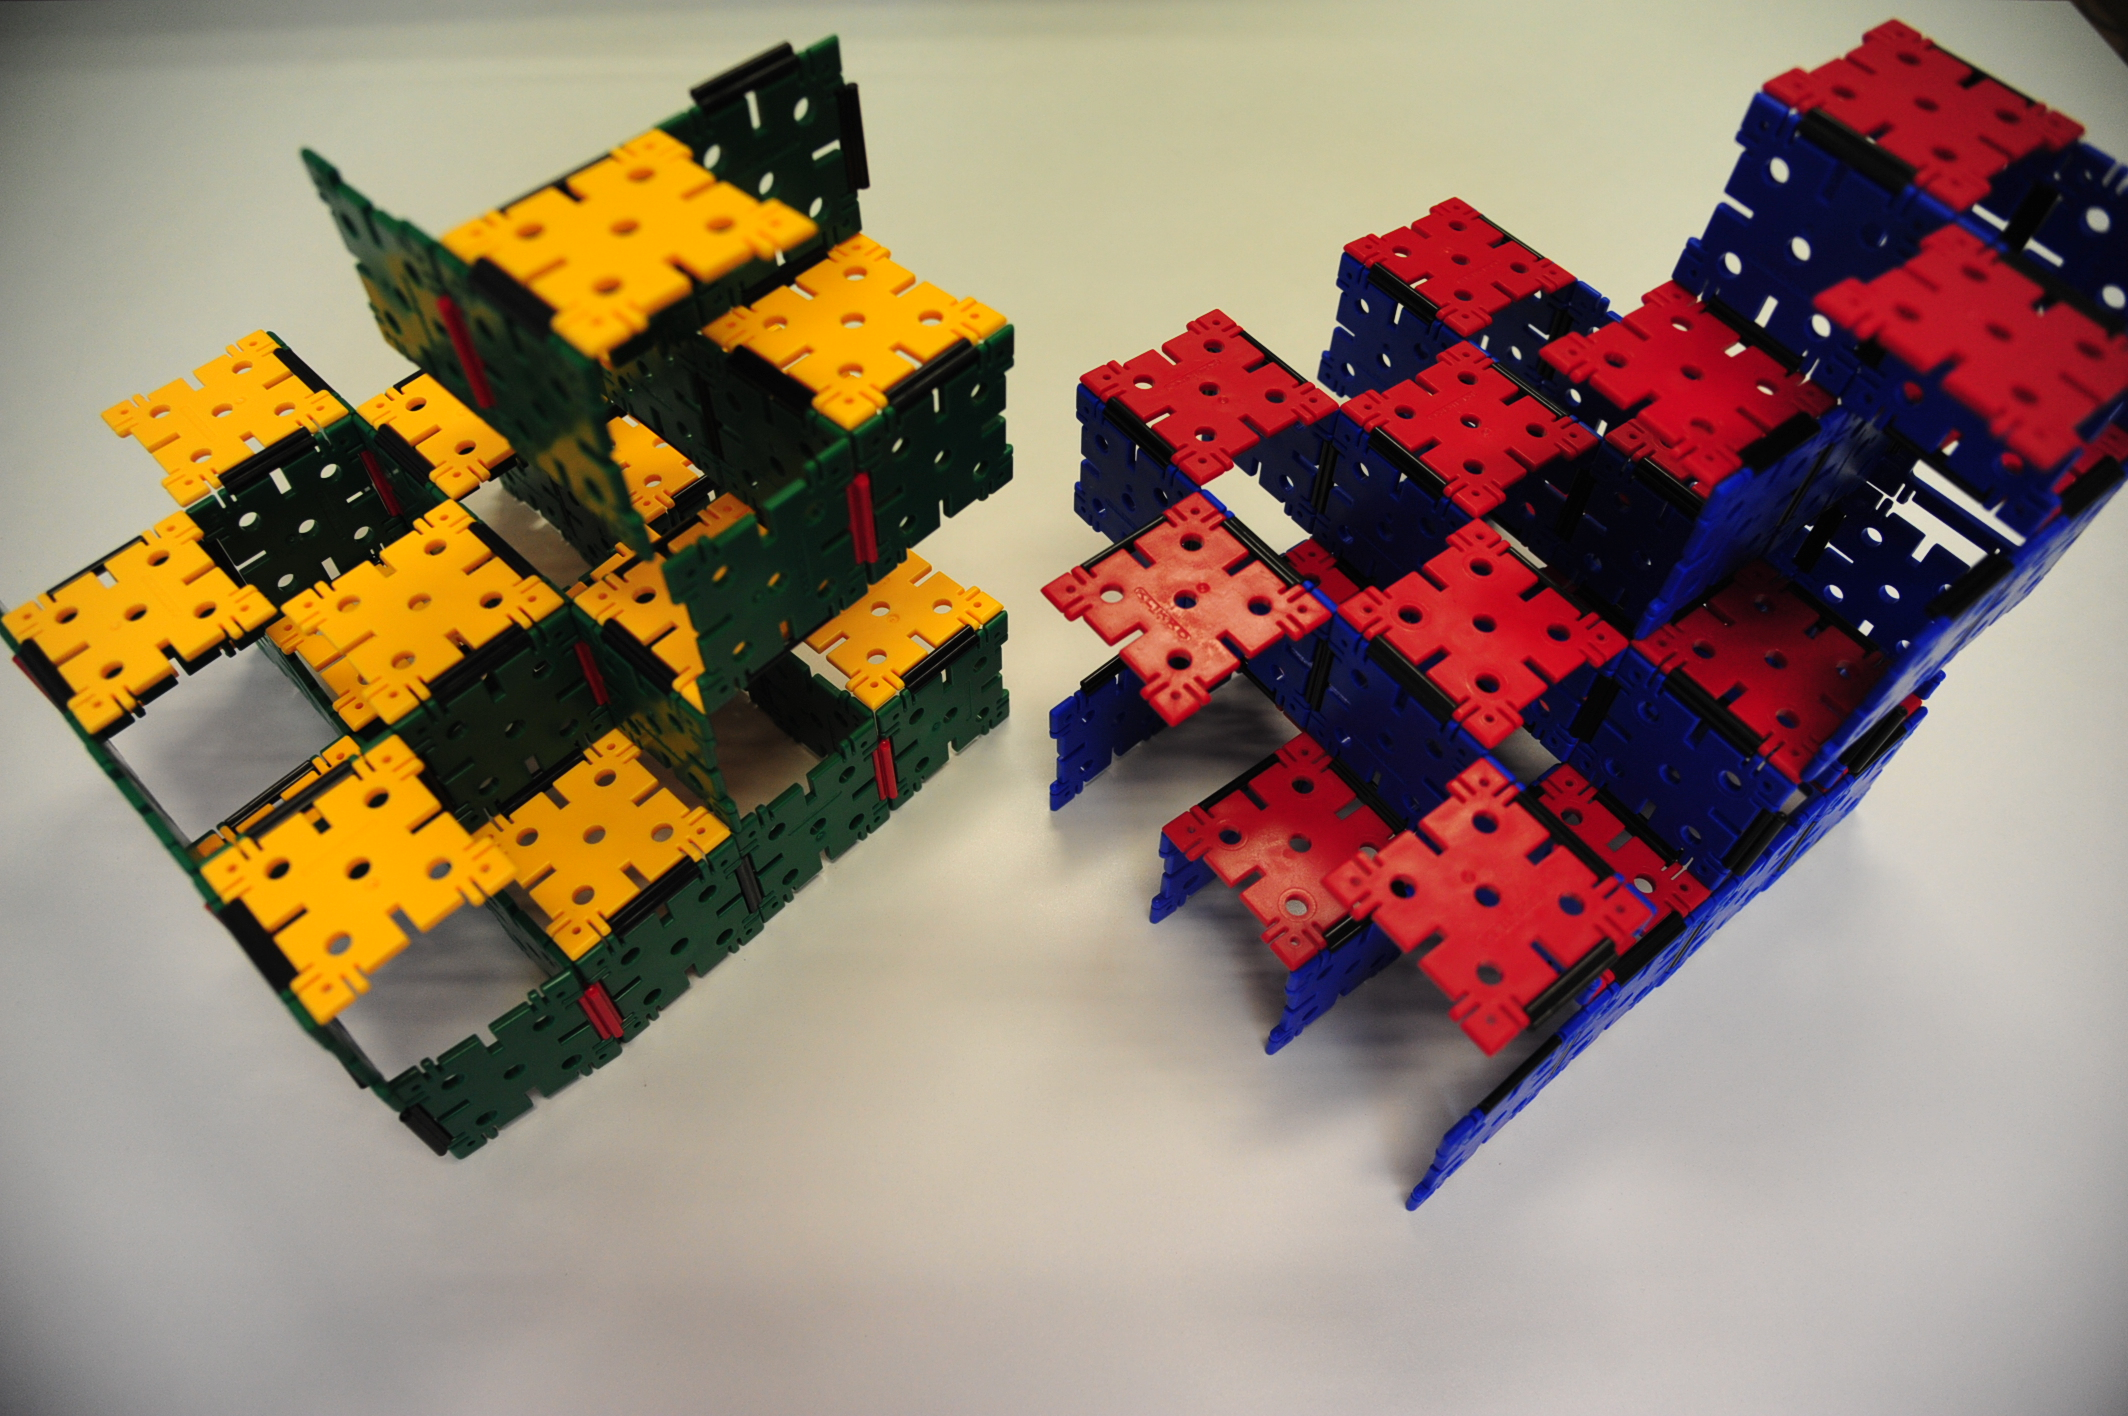
\includegraphics[height=4cm]{toys}
			%\end{center}
  \end{frame}
}


% Delete this, if you do not want the table of contents to pop up at
% the beginning of each subsection:

\begin{document}

\begin{frame}
  \titlepage
\end{frame}

\begin{frame}{Collaborators}
\begin{itemize}
%\item Yunqing Ouyang (欧阳云卿): Fudan University.
%\item Qing-Rui Wang (王晴睿): Chinese University of Hong Kong $\rightarrow$ Yale University.
%\item Zheng-Cheng Gu (顾正澄): Chinese University of Hong Kong.
\item Yunqing Ouyang: Fudan University.
\item Qing-Rui Wang: Tsinghua University.
\item Zheng-Cheng Gu: Chinese University of Hong Kong.
\begin{center}
	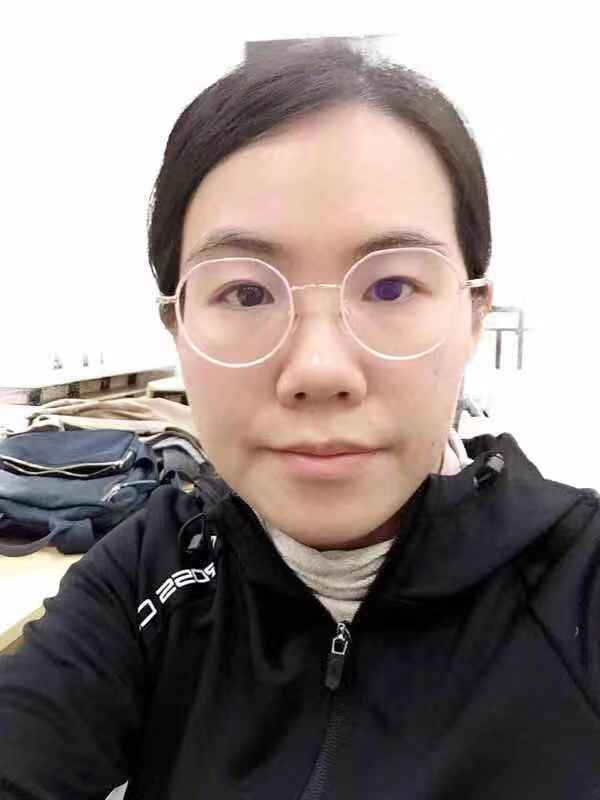
\includegraphics[height=3cm]{../people/yunqing}
	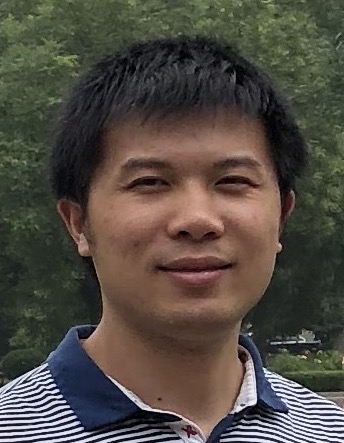
\includegraphics[height=3cm]{../people/qingrui}
	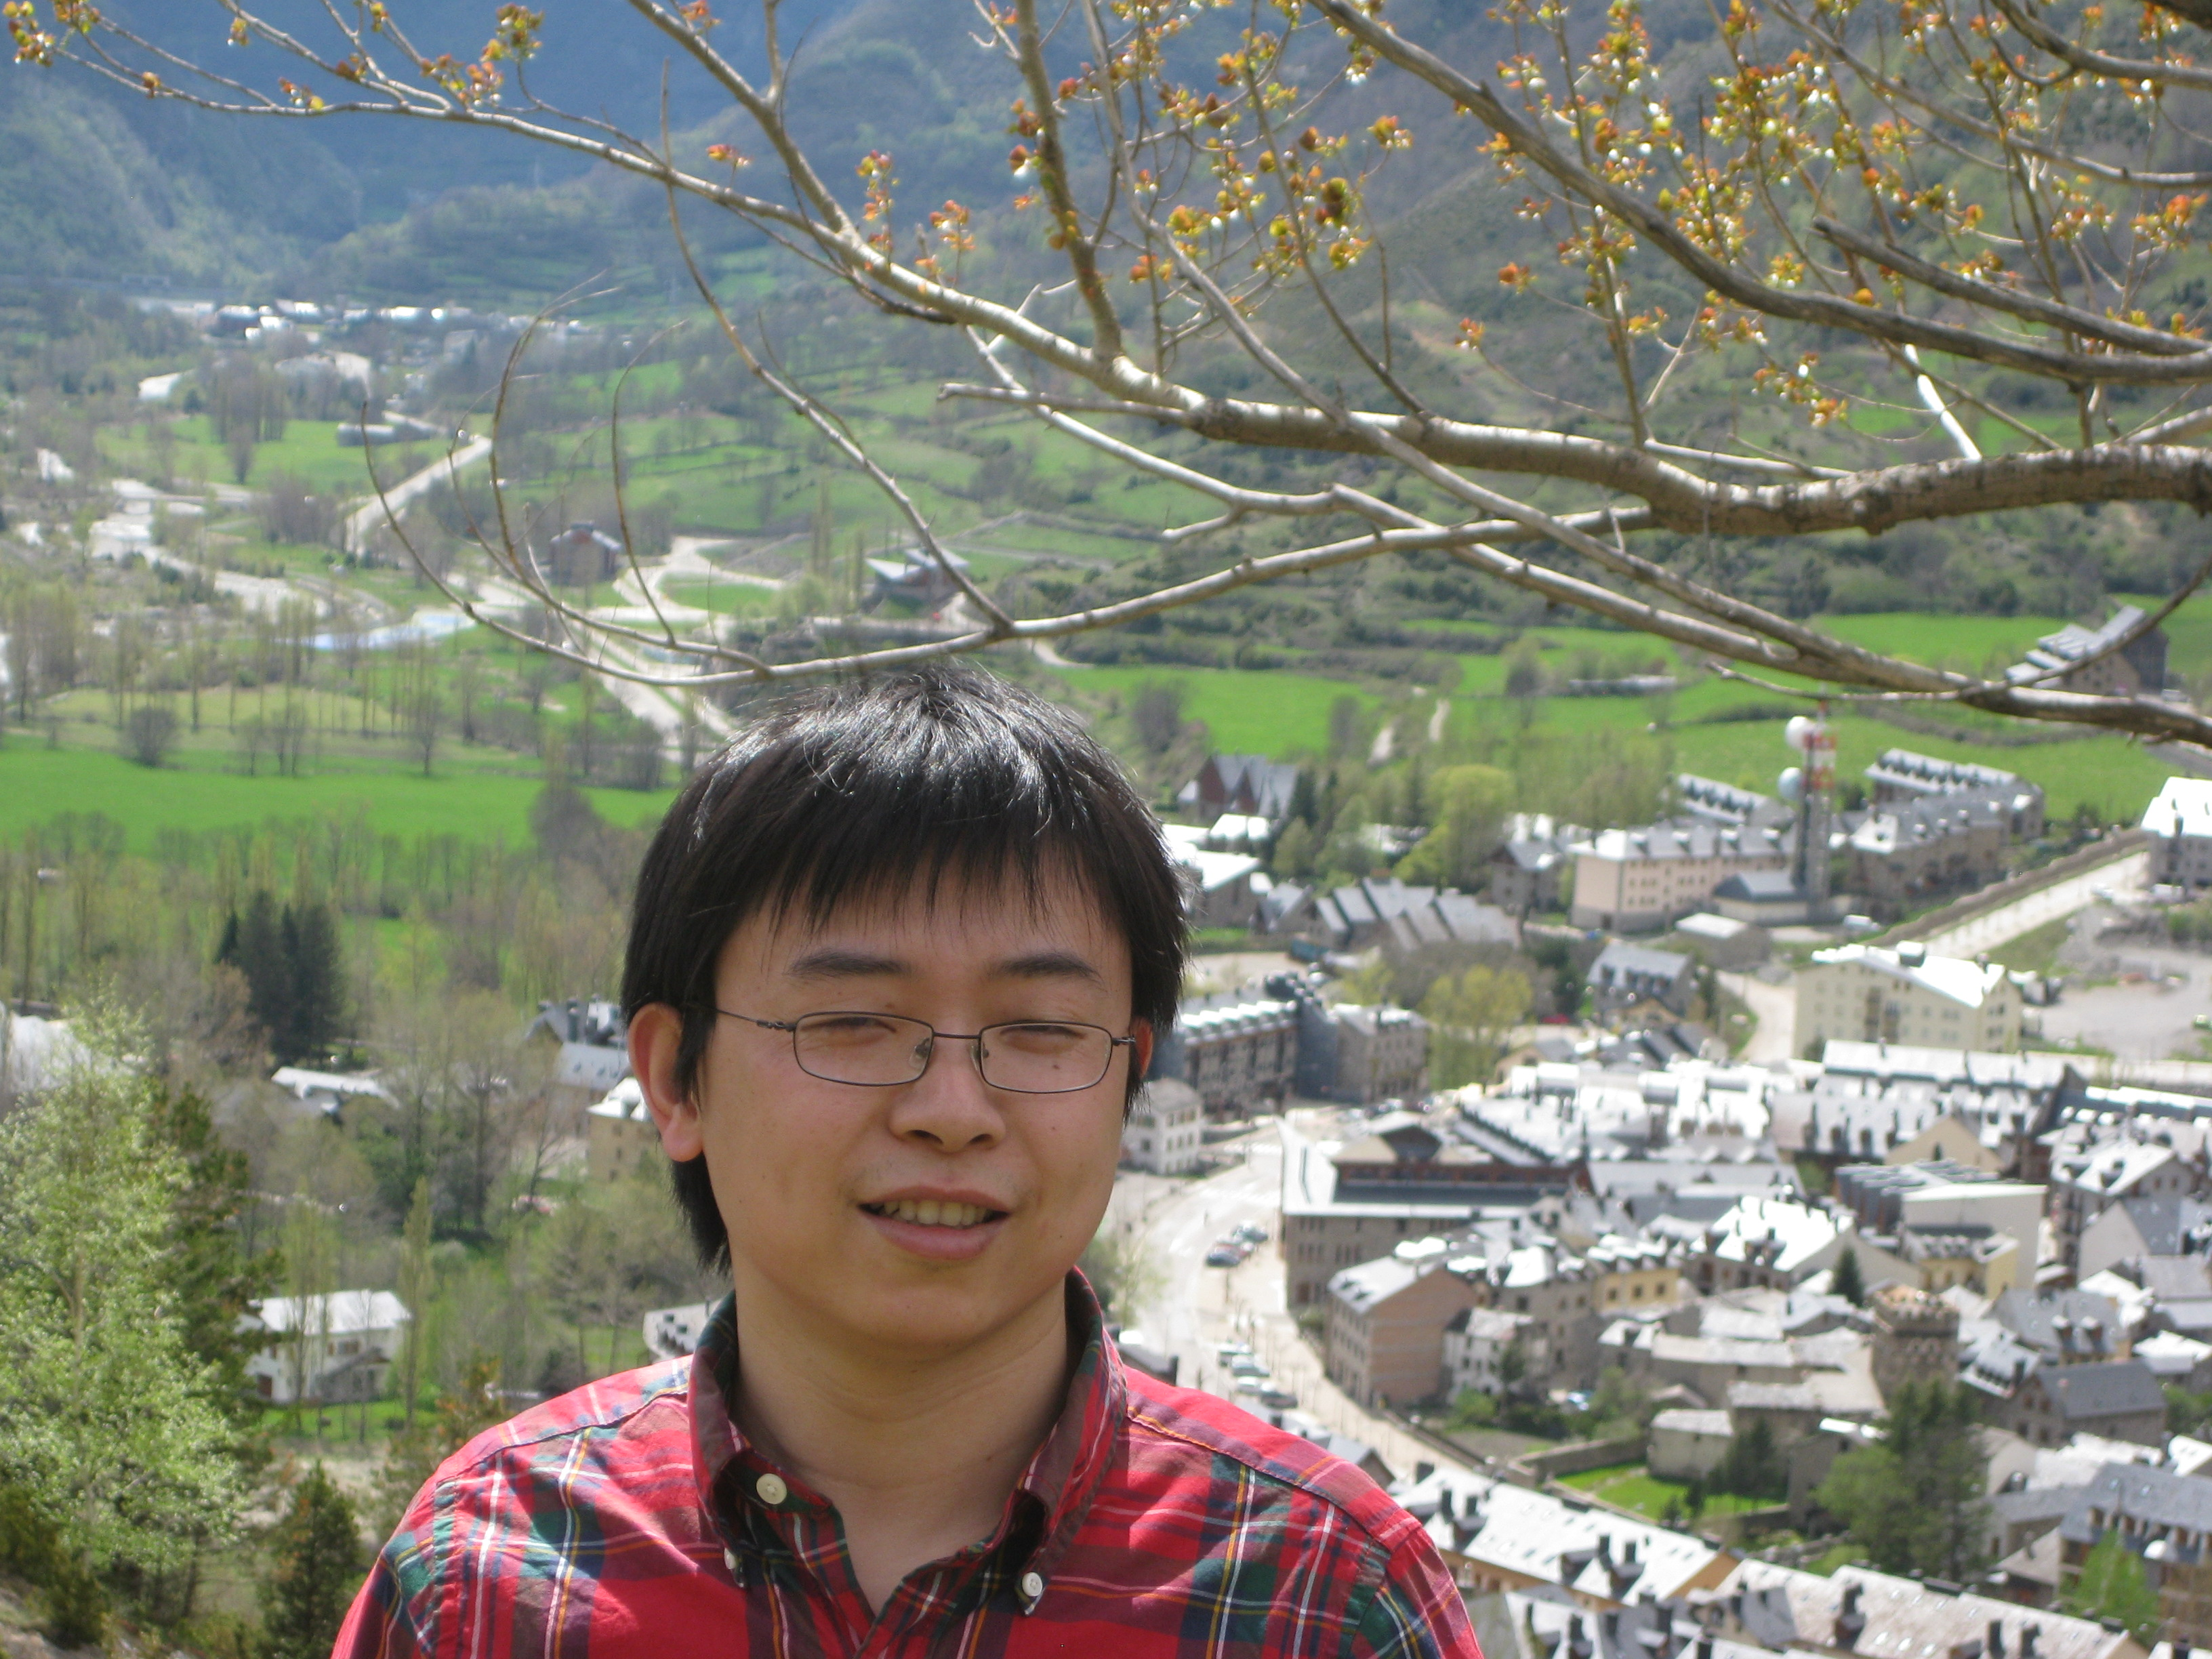
\includegraphics[height=3cm]{../people/zhengcheng}
\end{center}
\item Yunqing Ouyang, Qing-Rui Wang, Zheng-Cheng Gu and YQ,\\
Chin. Phys. Lett. \textbf{38}, 127101 (2021).
\item \url{https://github.com/yangqi137/SptSet}
\end{itemize}
\end{frame}

\section{Motivation: the problem we try to solve.}

\begin{frame}
  \frametitle{Symmetry-Protected Topological (SPT) states}
\begin{itemize}
\item SPT: gapped topological phases beyond Landau paradiam.
\item Cannot be smoothly connected to a trivial state without closing gap or breaking symmetry.
\item Symmetry-protected gapless surface states.
\item Free-fermion states: topological insulators, topological superconductors.
\item Bosonic SPTs: Haldane chain, CZX/Levin-Gu state, etc.\\
\emph{Xie Chen, Zheng-Cheng Gu, Zheng-Xin Liu and Xiao-Gang Wen, Science 2012.}
\item Interacting fermionic SPTs.
\end{itemize}
\begin{center}
	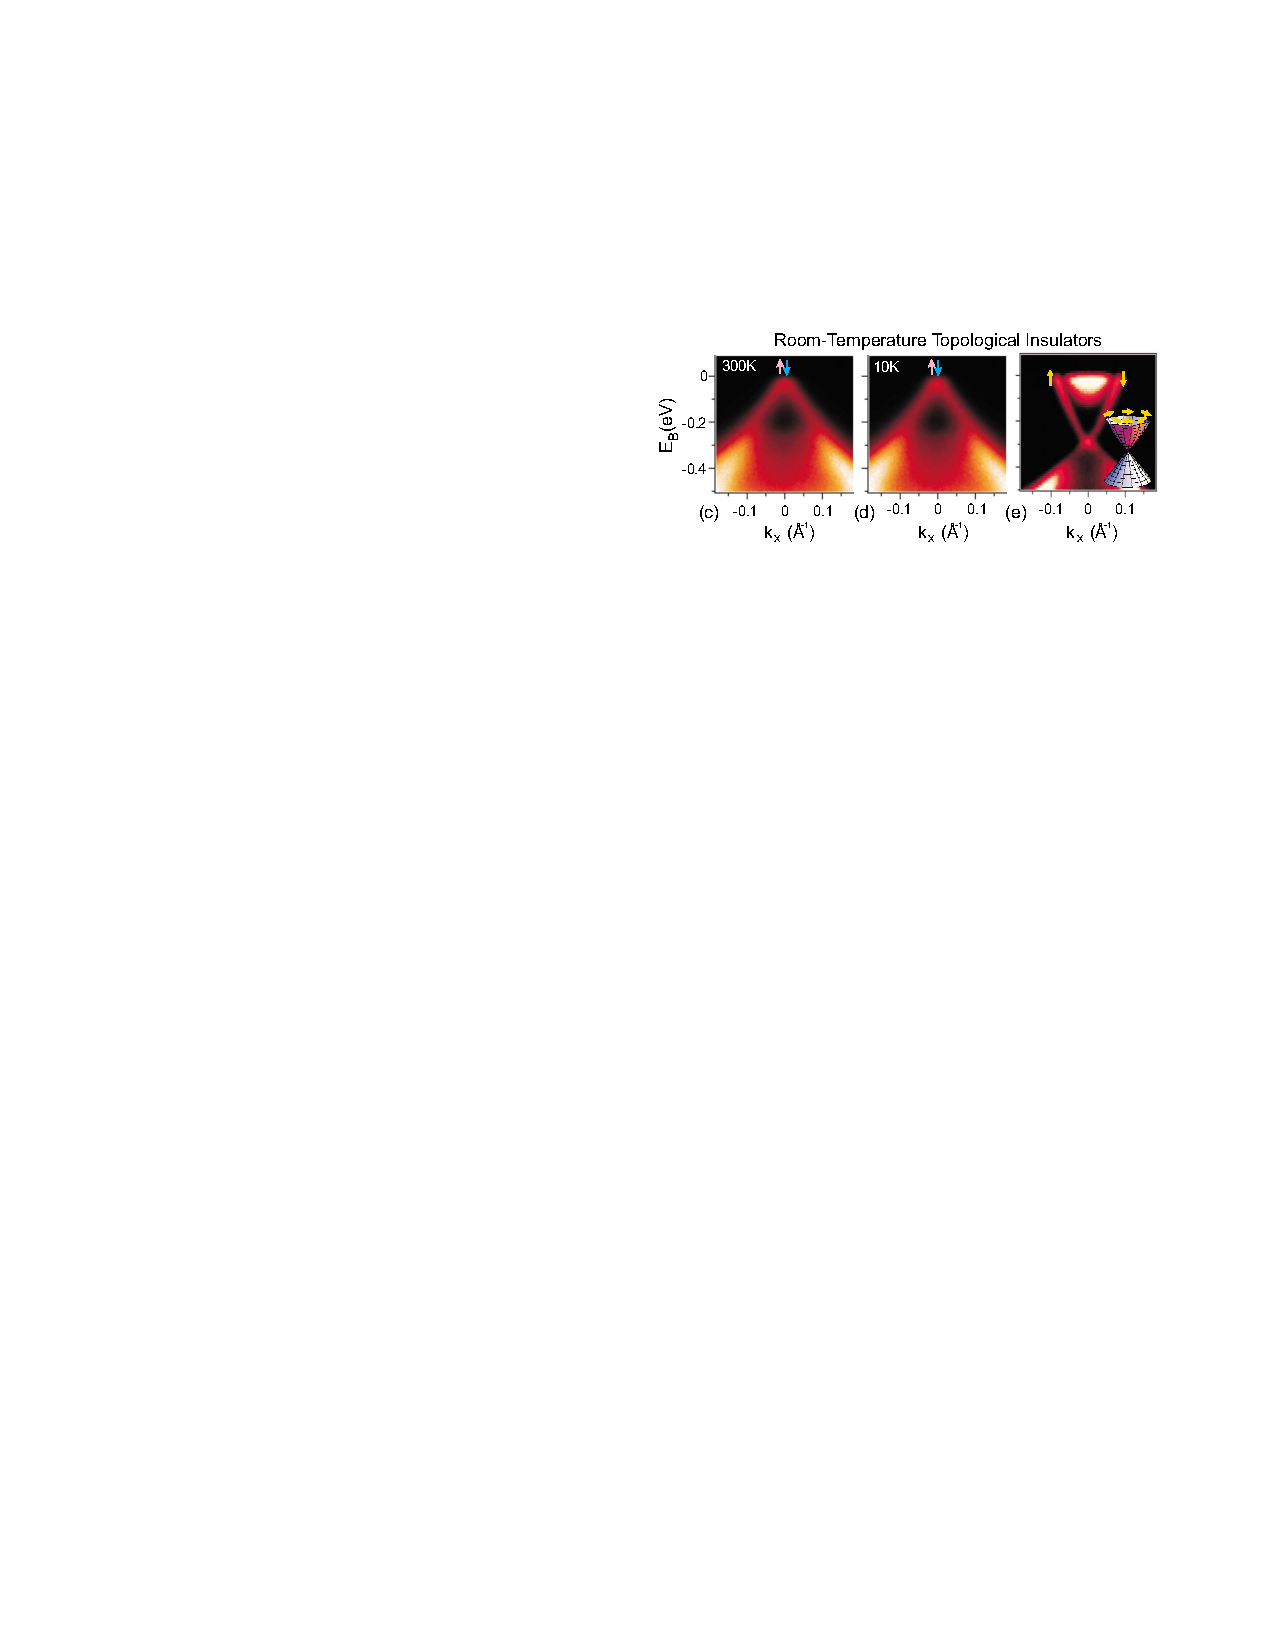
\includegraphics{../spspt/ti_surface}
\end{center}
\end{frame}

\begin{frame}
\frametitle{Bosonic SPT: Group Cohomology Theory}
\begin{itemize}
	\item \emph{Inhomogeneous} $n$-cochain $\omega: G^{\times n}\rightarrow \uone$\\
	We denote the space of $n$-cochains by $C^n[G,\uone]$.
	\item Define a coboundary operation $d^n:C^n[G,\uone]\rightarrow C^{n+1}[G,\uone]$
	\begin{align*}
		d\omega &(g_1,\ldots,g_{n+1})=g_1\cdot \omega(g_2,\ldots,g_n)
		-\omega(g_1g_2,\ldots,g_{n+1})
		+\omega(g_1,g_2g_3,\ldots,g_{n+1})\\
		&+\cdots+(-1)^i\omega(g_1,\ldots,g_ig_{i+1},\ldots,g_{n+1})
		+\cdots + (-1)^{n+1}\omega(g_1,\ldots,g_n).
	\end{align*}
	\item This forms a cochain complex:
	\[C^0\xrightarrow{d^0}C^1\rightarrow\cdots\rightarrow C^{n-1}\xrightarrow{d^{n-1}}C^n\xrightarrow{d^n}C^{n+1}\rightarrow\cdots\]
\end{itemize}
\end{frame}

\begin{frame}
	\frametitle{Bosonic SPT: Group Cohomology Theory}
	\begin{itemize}
		\item The cochain complex:
		\[C^0\xrightarrow{d^0}C^1\rightarrow\cdots\rightarrow C^{n-1}\xrightarrow{d^{n-1}}C^n\xrightarrow{d^n}C^{n+1}\rightarrow\cdots\]
		satisfying $d^2=0$ ($d^n\circ d^{n-1}=0$)
		\item We can define cohomology groups:
		\[H^n[G,\uone] = \frac{Z^n}{B^n} = \frac{\ker d^n}{\img d^{n-1}}.\]
		\item $(d+1)$-dimensional fixed-point partition functions are given by
		\[H^{d+1}[G,\uone].\]
	\end{itemize}
\end{frame}

\begin{frame}
  \frametitle{Fermionic SPT states}
  \begin{itemize}
  \item Atiyah–Hirzebruch Spectral Sequence for a generalized cohomology theory:
    \[E_2^{pq} = H^p(G, \mathcal H^q(*)) \Rightarrow \mathcal H^{p+q}(G).\]
    \begin{itemize}
    \item $\mathcal H^q(*)$: $q$-dimensional invertible topological order (iTO).
    \[\Omega^0=\uone_T,\quad\Omega^1=\mathbb Z_2,\quad\Omega^2=\mathbb Z_2,\quad\Omega^3=\mathbb Z_T.\]
    \item Physical interpretation: Decorate codim-$p$ DW w/ $(q+1)$-d iTOs.
    \end{itemize}
  \item Wave function: $\psi\in \Psi^d(G)$: $\psi=\begin{pmatrix}\psi^0&\psi^1&\cdots&\psi^{d+1}\end{pmatrix}$.
  \end{itemize}
  \begin{center}
    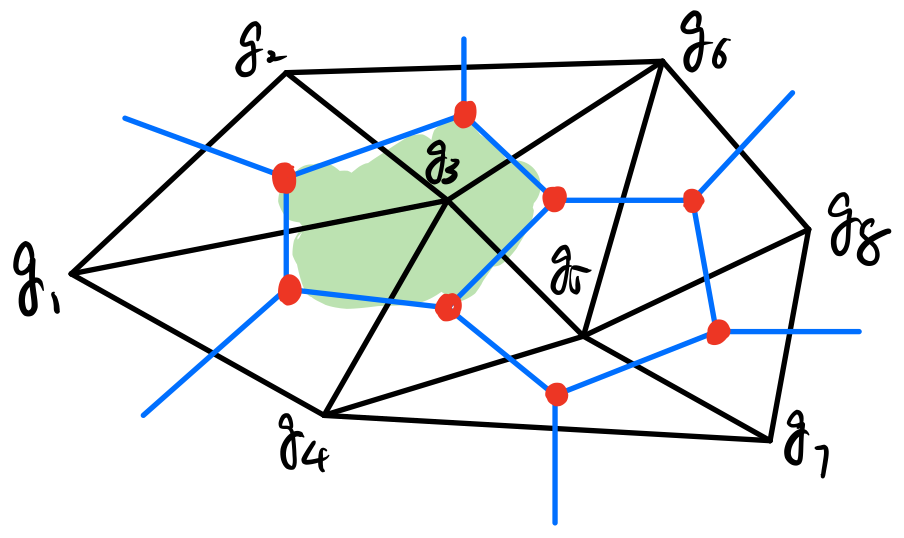
\includegraphics[height=3cm]{decoration}
  \end{center}
\end{frame}

\begin{frame}
  \frametitle{Symmetry group: $G$, $s$ and $\omega_2$}
  Symmetry is specified by three pieces of information:
    \begin{enumerate}
    \item (Bosonic) symmetry group $G$;
    \item Unitary/antiunitary structure: $s:G\rightarrow \mathbb Z_2$; Example: s(T)=1.
    \item $\omega_2\in H^2(G, \mathbb Z_2^f)$, classifying $1\rightarrow\mathbb Z_2^f\rightarrow G_f\rightarrow G\rightarrow1$. Example: $\omega_2(T, T)=\pm1$.
    \end{enumerate}
	$\mathcal H^{d+1}(G)$ depends on $(G, s, \omega_2)$.
\end{frame}

\begin{frame}
	\frametitle{Coboundary operation}
	\begin{itemize}
		\item Consider the coboundary of a single-layer state
		$\psi = \begin{pmatrix}0&\cdots&\psi^p&\cdots&0\end{pmatrix}$.
		\item $\delta\psi$ only contains layers $p'<p$:
		$\delta\psi=\begin{pmatrix}0&\cdots&d\psi^p&(\delta\psi)^{p+2}\cdots&(\delta\psi)^{d+2}\end{pmatrix}$.
		\item We denote $(\delta\psi)^{p'}=\mathcal D^{p, d-p+1}_{p'-p}(\psi^p)$.
		$D^{pq}_r:C^p(G_b,\Omega^q)\rightarrow C^{p+r}(G_b,\Omega^{q-r+1})$.
		\item $d$ is like an upper-triangular matrix.
		\item Examples: in 2d, $G=G_b\times\mathbb Z_2^f$
		\begin{align*}
			\mathcal D_2^{12} &= s\cup\psi^1\cup\psi^1,\\
		  \mathcal D_2^{21} &= \frac12\psi^2\cup\psi^2
		  +\frac12\psi^2\cup_1d\psi^2
		  +\mathcal O_4'(d\psi^2).
		\end{align*}
		\[  O_4'(\psi^2)(01234)
		  =\frac12d\psi^2(0124)d\psi^2(0234)
		  -\frac14\{d\psi^2(0123)[1-d\psi^2(0124)] \mod 2\}.\]
	\end{itemize}
\end{frame}

\begin{frame}
	\frametitle{Stacking operation}
	\begin{itemize}
		\item Not a simple component-wise addition:
		$\psi_1\boxplus\psi_2\neq (\psi_1^{d+1}+\psi_2^{d+1},\ldots,\psi_1^0+\psi_2^0)$.
		\item Reason: reordering of fermionic degrees of freedom.
		\item Result on the $p$-th layer will be twisted by higher layers.
		\[(\psi_1\boxplus\psi_2)^p = \psi_1^p + \psi_2^p
    + \mathcal A^{p,d-p+1}(\psi_1^{d+1},\psi_2^{d+1},\ldots,\psi_1^{p+1}, \psi_2^{p+1}),\]
		\item Examples: in 2d, $G=G_b\times\mathbb Z_2^f$
		\begin{align*}
		  \mathcal A^{21} &= \psi^1_1\cup\psi^1_2;\\
		  \mathcal A^{30} &= \frac12\psi^2_1\cup_1\psi^2_2 + \frac12 (\psi^1_1\cup\psi^1_2)\cup_1(\psi^2_1+\psi^2_2).
		\end{align*}
	\end{itemize}
	\begin{center}
		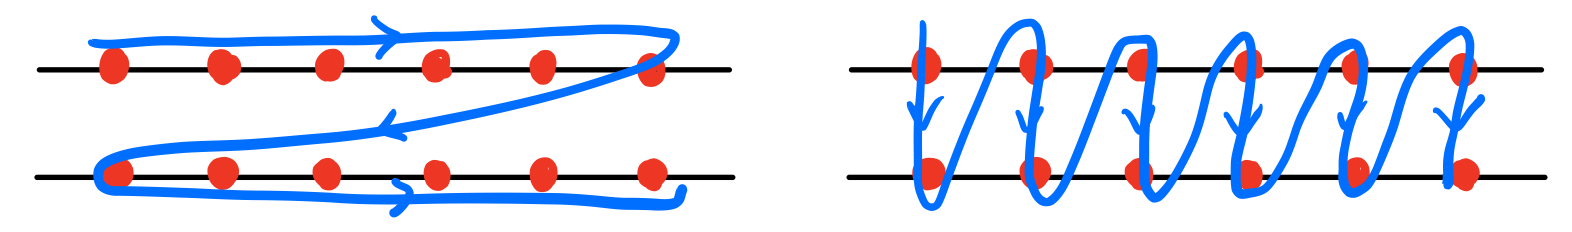
\includegraphics[height=2cm]{forder}
	\end{center}
\end{frame}

% \begin{frame}
% 	\frametitle{Fermionic SPT: a generalized cohomology theory}
% 	\begin{itemize}
% 		\item A spectral sequence: an fSPT state is specified by several layers.
% 		\item Example: 2D fSPT,
% 		\begin{enumerate}
% 			\item $n_1\in H^1[G, \mathbb Z_2]$: Majorana-chain decoration.
% 			\item $n_2\in C^2[G, \mathbb Z_2]$: Complex-fermion decoration.
% 			\item $\nu_3\in C^3[G, \uone]$: Bosonic phase factor.
% 		\end{enumerate}
% 		\item Obstruction functions: higher-page derivatives of the spectral sequence.
% 		\item Example: checking if $n_1\in H^1[G, \mathbb Z_2]$ is obstructed?
% 		\begin{enumerate}
% 			\item Check $\mathcal O_3[n_1] = \omega_2\cup n_1 + s_1\cup n_1\cup n_1$ vanishes.
% 			\item Find $n_2$ such that $dn_2 = \mathcal O_3[n1]$.
% 			\item Check $\mathcal O_4[n_2]$ vanishes.
% 			\begin{align*}\mathcal O_4(01234) = \frac12\big[\omega_2\cup n_2 + n_2\cup n_2 + n_2 \cup_1 dn_2 + \omega_2(013)dn_2(1234)\\ + dn_2(0124)dn_2(0234)\big]
% 			-\frac14\big\{dn_2(0123)[1-dn_2(0124)]\text{ (mod 2)}\big\}.
% 		\end{align*}
% 		\end{enumerate}
% 		This defines a map between cohomology classes
% 		$n_1\mapsto \mathcal O_4$.
% 		\item In theory, this is the end of the story. But in practice...
% 	\end{itemize}
% \end{frame}

\begin{frame}
	\frametitle{Computational cost}
	\begin{itemize}
		\item Key step: solving the cocycle/coboundary equation; finding $\ker d^n$ and $\img d^{n-1}$.
		\item ``Diagonalizing'' the coboundary matrix $d^n$: Smith Normal Form.
		\item $d^n$ acts on $\alpha(g_1,\ldots,g_n)$: $(|G|-1)^n$-dimension.
		\item Complexity = $O(N^3)$, $N = (|G|-1)^n$.
		\item Quite expensive for large $G$ ($|G| > 16$); infinite for $|G|=\infty$ (wallpaper and space groups).
	\end{itemize}
	\begin{block}{Can we do better?}
		\begin{itemize}
			\item For bSPTs: $H^n[G,\uone]$ can be computed using simpler $BG$.
			\item What about fSPTs and other cases w/ complicated maps b/w cohomology groups?
		\end{itemize}
	\end{block}
\end{frame}

\begin{frame}
	\frametitle{Other similar tasks}
	\begin{itemize}
		\item Symmetry-Enriched Topological (SET) states: ($\mathcal C^\times_G$)\\
		Maissam Barkeshli and Meng Cheng, arXiv:1906.10691.

		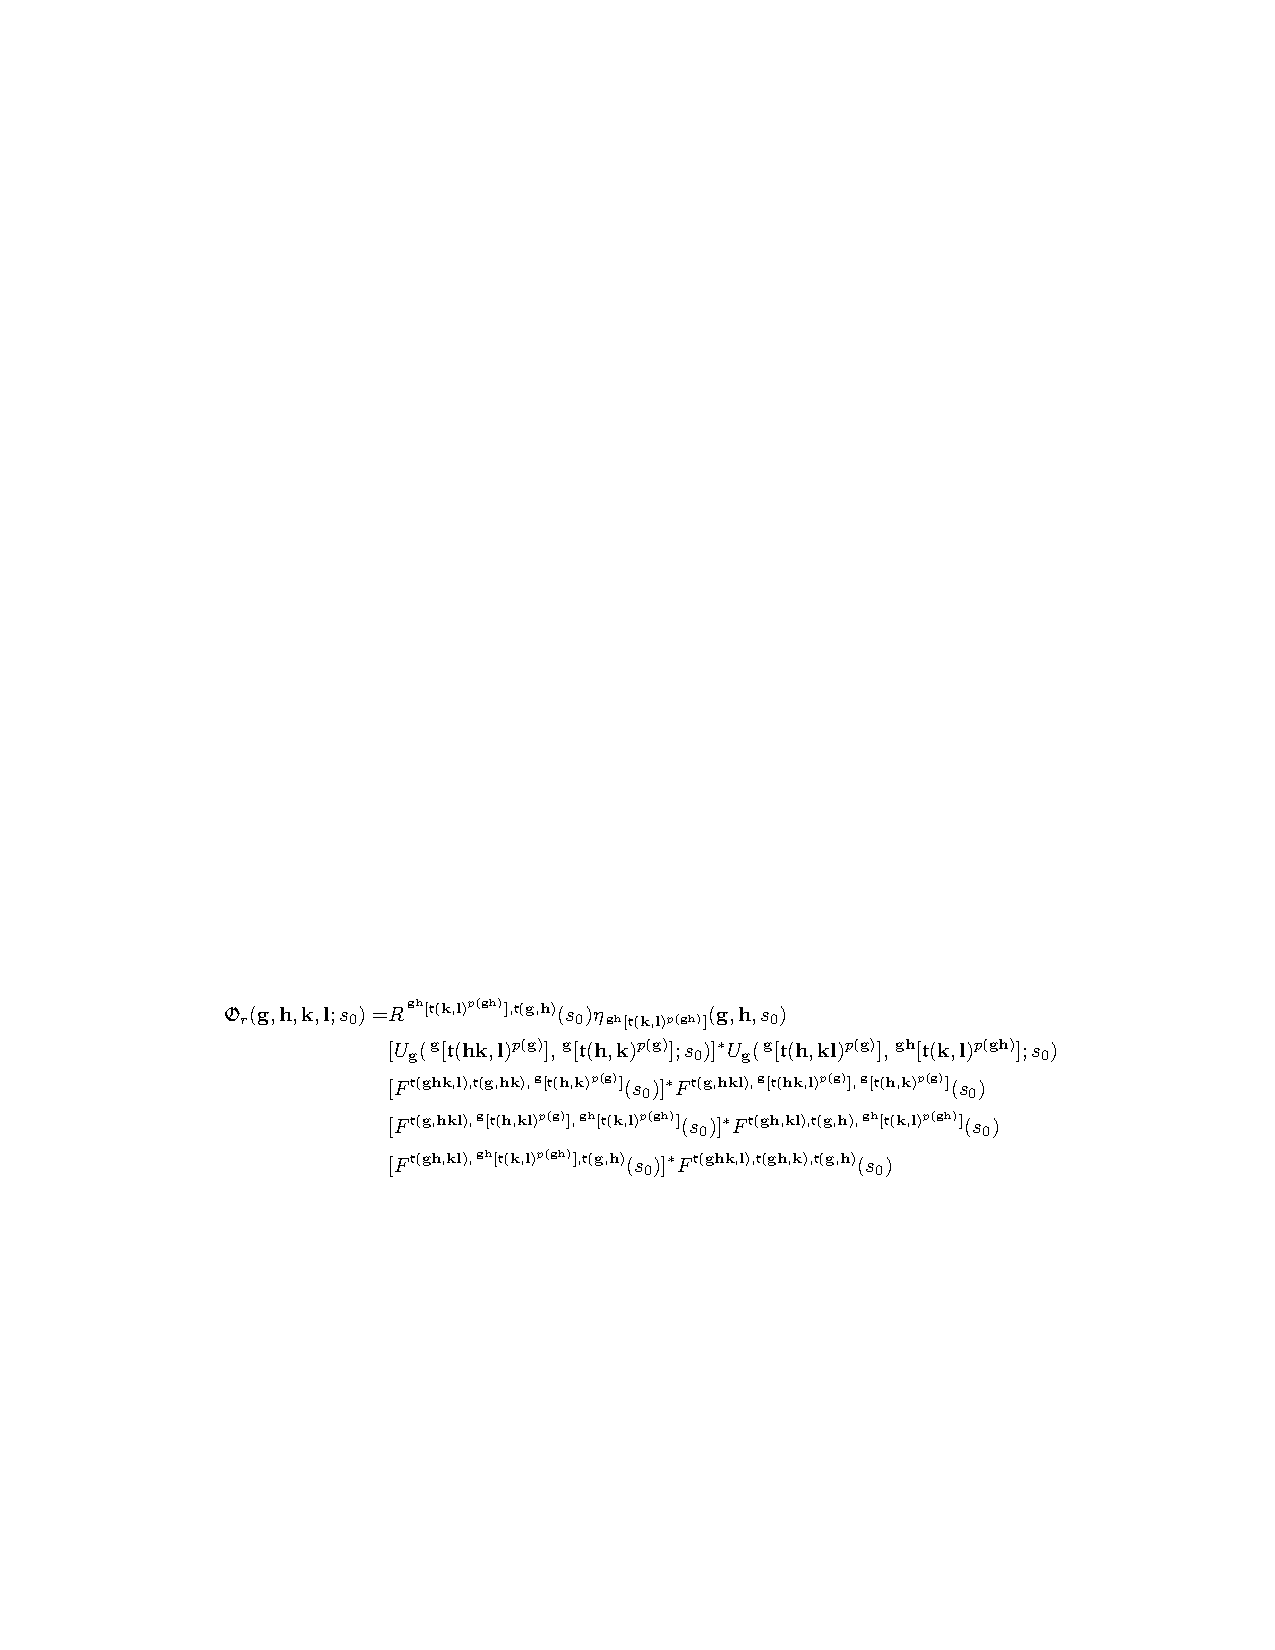
\includegraphics[scale=.8]{relanomaly_eq}
		\item 3D U(1) spin liquids:\\
		Shang-Qiang Ning, Liujun Zou and Meng Cheng, arXiv:1905.03276.

		
\includegraphics[scale=.8]{u1sl_eq}
	\end{itemize}
\end{frame}

\begin{frame}
	\frametitle{Our goal}
	\begin{itemize}
		\item Our goal: develop an algorithm to accelerate the computation of cohomology groups of $G$ and mapping between cohomology groups.
		\item Why we want a faster computation?
		\begin{enumerate}
			\item fSPT: Some nontrivial decorations and decorations only appear for complicated $G$.
			\item Realistic system: crystalline-symmetry groups $|G|=\infty$.
		\end{enumerate}
		\item We want to develop an easy-to-use software package for computing fSPT and SET classifications.
		\item A live demo of what we have now...
	\end{itemize}
\end{frame}

\section{Picture: using a simplified model of the classifying space.}

\begin{frame}
	\frametitle{Classifying space, cocycles and bSPT-state partition functions}
	\begin{itemize}
		\item In algebraic topology:
		$H^D[G, \uone] = H^D[BG, \uone]$.
		\item BG: a topological space satisfying $\pi_1(BG)=G$, $\pi_n(BG)=0$ for $n\geq 2$.
		\item Intuitive picture: $BG$ is like an altas.
		\item Cochain: $\alpha\in \hhom[X_n(BG), \uone]$, $\alpha; \alpha(g_1);\alpha(g_1,g_2);\alpha(g_1,g_2,g_3);\cdots$.
	\end{itemize}
	\begin{center}
		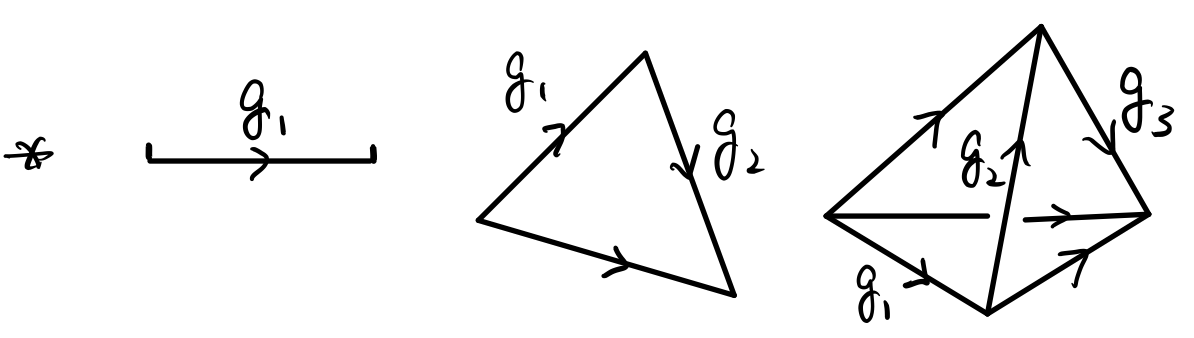
\includegraphics[width=10cm]{bg-std}
	\end{center}
\end{frame}

\begin{frame}
	\frametitle{Classifying space, cocycles and bSPT-state partition functions}
	\begin{itemize}
		\item
		$\alpha$ = a partition function $Z_\alpha$ of an SPT phase.
		\item Evaluating $Z_\alpha$ on a $G$-bundle:
		\begin{enumerate}
			\item Make a triangulation of the $G$-bundle;\\
			\emph{Coverting $G$ with cells in $BG$}
			\item Assign to each simplex (\emph{cell}) a phase
			$\alpha(g_1,g_2,\ldots,g_{d+1})$;
			 \emph{This can always be done because $BG$ is the (base space of the) universal $G$-bundle.}
			\item Add all phases together,
			\[Z_\alpha(M) = \exp\{2\pi \sum_{\Delta}s_\Delta\alpha(g_{i_1},g_{i_2})\}.\]
		\end{enumerate}
	\end{itemize}
	\begin{center}
		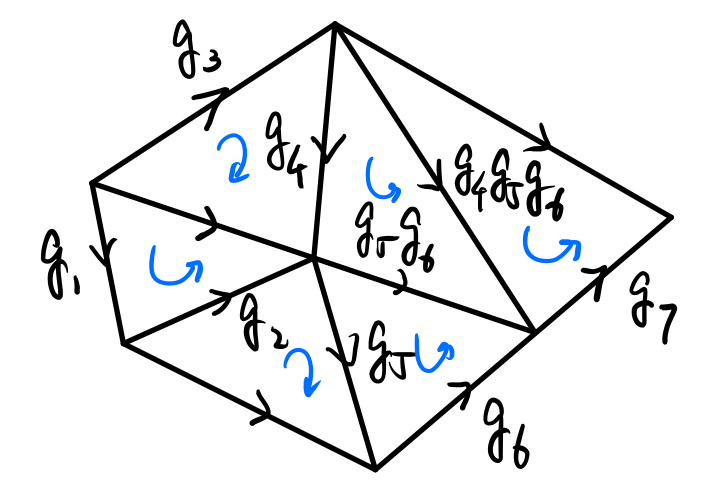
\includegraphics[height=3cm]{tri-orient}
	\end{center}
\end{frame}

\begin{frame}
	\frametitle{A standard and a simplified construction of $BG$}
	\begin{enumerate}
		\item Standard construction: $BG$ as a simplicial complex.
		\begin{itemize}
			\item All cells are simplices, $[g_1|g_2|\cdots|g_n]$.
			\item Uniform boundary operations:
			$\partial[g_1|g_2]=g_1[g_2]-[g_1g_2]+[g_1]$, ...
			\item Requires many cells.
		\end{itemize}
		\item Simplified construction: $BG$ as a CW-complex.
		\begin{itemize}
			\item Cells have arbitrary shapes.
			\item Arbitrary boundary operations.
			\item Can have very few cells.
		\end{itemize}
	\end{enumerate}
	\begin{center}
		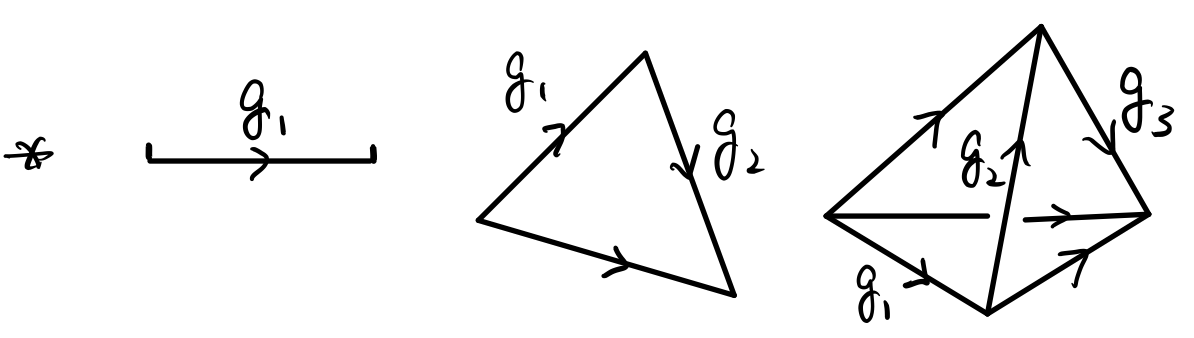
\includegraphics[width=10cm]{bg-std}~~~~
		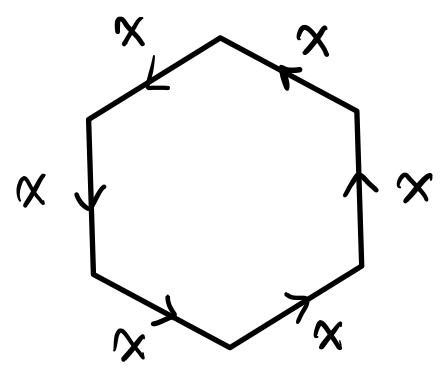
\includegraphics[height=3cm]{z6-1}
	\end{center}
\end{frame}

\begin{frame}
	\frametitle{Computing the group cohomology using $BG$}
	\begin{itemize}
		\item $H^D[G, \uone] = H^D[BG, \uone]$: need to compute the cohomology group of $BG$.
		\item The coboundary operator $d^n$ is a matrix of size $|X_n(BG)|\times |X_{n+1}(BG)|$.
		\item Complexity: $|X_n(BG)|^3$.
		\item It is much easier to compute for the simplified $BG$.
		\item $BG$ is actually simple when $G$ is infinite but torsion-free:
		$B\mathbb Z=S^1$, $B\mathbb Z^2=T^2$, etc.
	\end{itemize}
\end{frame}

\begin{frame}
	\frametitle{How to compute cohomology operations}
	\begin{itemize}
		\item Consider $f: H^p[G,\uone]\rightarrow H^{p'}[G, \uone]$.
		\item In general, we do not know how to derive the formula for a simplified $BG$.
		\item Map to/from the standard $BG$: a dictionary translating b/w two types of cohomology classes.
		\[H^p[BG_1,\uone]\simeq H^p[BG_2,\uone].\]
		\item Algorithm:
		\begin{enumerate}
			\item Consider $\alpha$ on simplified $BG$.
			\item Convert to $\bar\alpha$ on standard $BG$.
			\item Compute $\bar\beta = f(\bar\alpha)$ using existing formula.
			\item Map $\bar\beta$ to $\alpha$ on the simplified $BG$.
			\item Check whether $\alpha$ is trivial.
		\end{enumerate}
	\end{itemize}
\end{frame}

\begin{frame}
	\frametitle{Example: cyclic group}
	\begin{itemize}
		\item Any two models of $BG$ are homotopic to each other. $BG_1\leftrightarrow BG_2$.
		\item Mapping: express cells in $BG_1$ using cells in $BG_2$.
		\item Example: $G=\mathbb Z_6$, $BG$ contains only one 2-cell.
		\item Map from standard to simplified:
		\[\alpha(e^2) = \bar\alpha(1, x)+\bar\alpha(x, x)
		+\cdots+\bar\alpha(x^5, x).\]
		\item The other direction: harder to draw, but can also be computed.
	\end{itemize}
	\begin{center}
		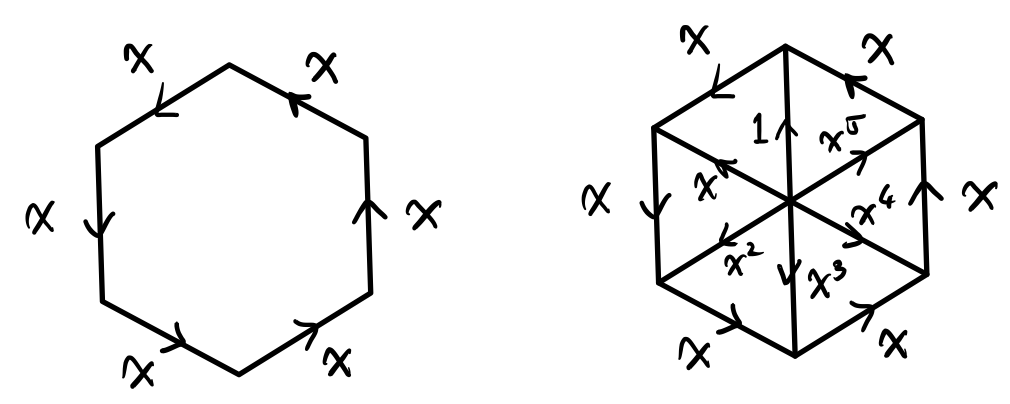
\includegraphics[height=3cm]{z6}

		{\footnotesize Acknowledgement: idea from Hao Zheng.}
	\end{center}
\end{frame}

\section{Algorithm: an algebraic tool from homology algebra.}

\begin{frame}
	\frametitle{Algebraic version: resolution}
	\begin{itemize}
		\item We do not need that much of geometric information of $BG$.
		\item Chain complex (augmented) of $EG$ ($EG/G=BG$)
		\[\cdots\rightarrow C_k(EG)\xrightarrow{\partial_k}
		C_{k-1}(EG)\rightarrow\cdots\rightarrow
		C_1(EG)\xrightarrow{\partial_1}
		C_0(EG)\xrightarrow{\epsilon}\mathbb Z\rightarrow0.\]
		\item Free resolution:
		\[\cdots\rightarrow F_k\xrightarrow{\partial_k}
		F_{k-1}\rightarrow\cdots\rightarrow
		F_1\xrightarrow{\partial_1}
		F_0\xrightarrow{\epsilon}\mathbb Z\rightarrow0.\]
		\item Forms a long exact sequence of free $\mathbb ZG$-modules.
		\item Cochain: $C^k=\hhom_G[F_k, \uone]$
		\item Coboundary: $d^n:C^n\rightarrow C^{n+1}$, $d^n\alpha(x) = \alpha(\partial x)$.
		\item Cohomology group: $H^n[G, \uone]=\frac{\ker d^n}{\img d^{n-1}}$.
	\end{itemize}
\end{frame}

\begin{frame}
	\frametitle{Example: bar resolution and inhomogeneous cocycle}
	\begin{itemize}
		\item Consider the (normalized) bar resolution:
		$F_n$ is generated by $[g_1|\cdots|g_n]$.
		\item Boundary map:
		\[\partial[g_1|\cdots|g_n]=g_1[g_2|\cdots|g_n]
		-[g_1g_2|\cdots|g_n]+[g_1|g_2g_3|\cdots|g_n]-\cdots.\]
		\item This gives the inhomogeneous cocycle:
		$\alpha([g_1|\cdots|g_n])=\alpha(g_1,\ldots,g_n)$.
		\item This corresponds to the standard construction of $BG$.
	\end{itemize}
\begin{center}
	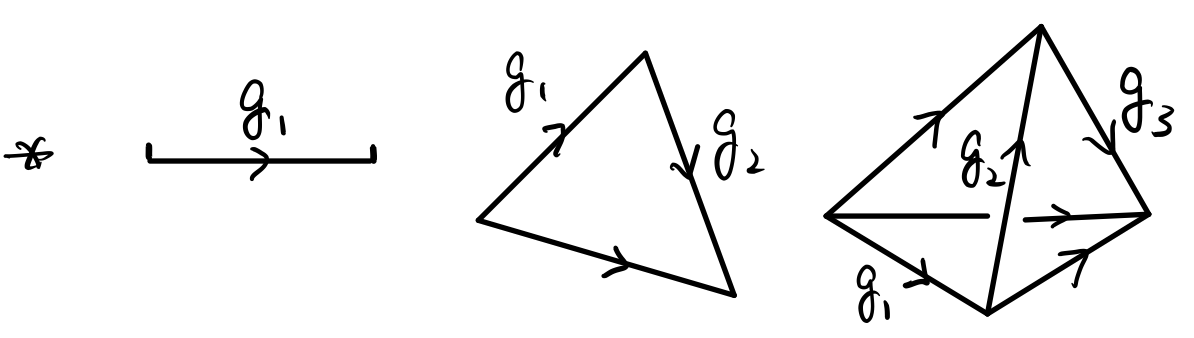
\includegraphics[width=10cm]{bg-std}
\end{center}
\end{frame}

\begin{frame}[fragile]
	\frametitle{Chain map between two resolutions}
	\begin{itemize}
		\item Consider two resolutions: simplified resolution $F$ and bar resolution $F'$.
		\item We can construct chain maps $f:F\rightarrow F'$ and $g:F'\rightarrow F$, such that
		\[\begin{tikzcd}
		\cdots\arrow[r,"\partial_{k+1}"]&
		F_k\arrow[r,"\partial_k"]\arrow[d,"f_k"]&
		F_{k-1}\arrow[r,"\partial_{k-1}"]\arrow[d,"f_{k-1}"]&
		\cdots\arrow[r,"\partial_2"]&
		F_1\arrow[r,"\partial_1"]\arrow[d,"f_1"]&
		F_0\arrow[r,"\epsilon"]\arrow[d,"f_0"]&
		\mathbb Z\arrow[d,"\id"]\\
		\cdots\arrow[r,"\partial_{k+1}'"]&
		F_k'\arrow[r,"\partial_k'"]&
		F_{k-1}'\arrow[r,"\partial_{k-1}"]&
		\cdots\arrow[r,"\partial_2'"]&
		F_1'\arrow[r,"\partial_1'"]&
		F_0'\arrow[r,"\epsilon'"]&
		\mathbb Z
		\end{tikzcd}\]
		commutes.
		\item $f^\ast$ and $g^\ast$ maps between two types of cocycles:
		\[f^\ast:C^{n\prime} = \hhom_G[F^\prime_n,\uone]\rightarrow C^n=\hhom_G[F_n,\uone]:
		f^\ast\alpha(x)=\alpha(f(x)).\]
	\end{itemize}
\end{frame}

\begin{frame}[fragile]
	\frametitle{Use chain maps to compute comohomogy operations}
	\begin{itemize}
		\item We want to compute a map $C^m\rightarrow C^n$.
		\item We only know the formula $C^{m\prime}\rightarrow C^{n\prime}$.
		\item Use $f^\ast$ and $g^\ast$:
	\end{itemize}
	\[\begin{tikzcd}
		C^m\arrow[r,dashrightarrow]\arrow[d,"g^\ast"] & C^n\\
		C^{m\prime}\arrow[r] & C^{n\prime}\arrow[u,"f^\ast"]
	\end{tikzcd}\quad\quad\quad
	\begin{tikzcd}
		\alpha\arrow[d,"g^\ast",mapsto] & \beta\\
		\alpha'\arrow[r,mapsto] & \beta'\arrow[u,"f^\ast",mapsto]
	\end{tikzcd}
	\]
\end{frame}

\begin{frame}[fragile]
	\frametitle{Contracting homotopy of a resolution}
	\begin{itemize}
		\item Since $F$ is a long exact sequence, we can construct a contracting homotopy: $\id:F\rightarrow F$ is homotopic to $0:F\rightarrow F$.
		\item A contracting homotopy $s_k: F_k\rightarrow F_{k+1}$
		\[
		\begin{tikzcd}
		F_{k+1} \arrow[r,"\partial_{k+1}"]
		&F_k\arrow[r,"\partial_k"]
		\arrow[d,"\id"]
		\arrow[ld,"s_k"]&
		F_{k-1}\arrow[ld,"s_{k-1}"]\\
		F_{k+1} \arrow[r,"\partial_{k+1}"]& F_k\arrow[r,"\partial_k"]&
		F_{k-1}
		\end{tikzcd}
		\]
		such that $\partial_{k+1}s_k + s_{k-1}\partial_k = \id$.
		\item $s$ can be used to compute the preimage of $\partial$: If $\partial x=0$, then $\partial s(x) = x$.
		\item For the bar resolution, $s(g_0[g_1|\cdots|g_n])
		=[g_0|g_1|\cdots|g_n]$.
		\item In practice, $s$ is constructed along with the simplified resolution $F$.
	\end{itemize}
\end{frame}

\begin{frame}[fragile]
	\frametitle{Constructing the chain map}
	\begin{itemize}
		\item We construct the chain map recursively,
		\[\begin{tikzcd}
		\cdots\arrow[r,"\partial_5"]&
		F_4\arrow[r,"\partial_4"]\only<6->{\arrow[d,"f_4"]}&
		F_3\arrow[r,"\partial_3"]\only<5->{\arrow[d,"f_3"]}&
		F_2\arrow[r,"\partial_2"]\only<4->{\arrow[d,"f_2"]}&
		F_1\arrow[r,"\partial_1"]\only<3->{\arrow[d,"f_1"]}&
		F_0\arrow[r,"\epsilon"]\only<2->{\arrow[d,"f_0"]}&
		\mathbb Z\arrow[d,"\id"]\\
		\cdots\arrow[r,"\partial_5'"]&
		F_4'\arrow[r,"\partial_4'"]&
		F_3'\arrow[r,"\partial_3"]&
		F_2'\arrow[r,"\partial_2'"]&
		F_1'\arrow[r,"\partial_1'"]&
		F_0'\arrow[r,"\epsilon'"]&
		\mathbb Z
		\end{tikzcd}\]
		\item In each step:
		\begin{columns}
			\column{.3\columnwidth}
			\[\begin{tikzcd}
			F_{n+1}\arrow[r,"\partial"]\arrow[d,"f_{n+1}",dashrightarrow]
			&F_n\arrow[d,"f_n"]\\
			F_{n+1}'\arrow[r,"\partial'"]&F_n'
			\end{tikzcd}\]
			\column{.7\columnwidth}
			\begin{enumerate}
				\item Choose a $\mathbb ZG$ basis $e^{n+1}_i$.
				$\partial'f_{n+1}(e^{n+1}_i) = f_n(\partial e^{n+1}_i).$
				\item Let $f_{n+1}(e^{n+1}_i)=s'(f_n(\partial e^{n+1}_i))$.
				\item Extend $f_{n+1}$ linearly to $F_{n+1}$.
			\end{enumerate}
		\end{columns}
	\end{itemize}
\end{frame}

\begin{frame}
	\frametitle{Constructing a simplified resolution}
	\begin{enumerate}
		\item Using the HAP package in the GAP software: \url{www.gap-system.org}.\\
		G. Ellis, J. Symb. Comput. \textbf{38}, 1077 (2004).
		\item Simple resolution for Abelian groups $\mathbb Z_n$.
		\item Wall's construction: CTC Wall, Math. Proc. Cam. Phil. Soc. \textbf{57}, 251 (1961).\\
		Given a group extension $1\rightarrow N\rightarrow G\rightarrow Q\rightarrow 1$, and resolutions of $N$ and $Q$: $F_N$ and $F_Q$, a resolution of $G$ can be constructed as a ``perturbation'' of $F_N\otimes F_Q$.
		\item Use Wall's construction, we can compute a simplified resolution for $G$ if $G$ is written as a series of group extensions:
		\[G=G_1\supset G_2\supset\cdots\supset G_n=\mathbb Z_1\]
		such that $G_i/G_{i+1}=\mathbb Z_{m_i}$ or $\mathbb Z$.\\
		This method works for all wallpaper and space groups.
	\end{enumerate}
\end{frame}

\begin{frame}
	\frametitle{Lazy evaluation}
	\begin{itemize}
		\item Lasy evaluation: compute $\alpha(g_1,\ldots,g_n)$ only when it is needed.
		\item Allows computation for $|G|=\infty$.
		\item Scheme:
		\[\alpha(e^4_i)\Rightarrow \alpha(g_1,g_2,g_3,g_4)
		\Rightarrow \frac12\beta(g_1,g_2)\beta(g_3,g_4)\Rightarrow \beta(e^2_j).\]
	\end{itemize}
	\begin{center}
		
\includegraphics[height=3cm]{geyou}
	\end{center}
\end{frame}

\begin{frame}[fragile]
	\frametitle{A subtlety: how to solve a cocycle equation}
	\begin{itemize}
		\item Task: given inhomogeneous cocycle $\beta'$, find solution $\alpha'$ such that $d\alpha'=\beta'$
		\item Use $f:F\rightarrow F'$ and $g:F'\rightarrow F$.
		\item Naively: $\beta'\Rightarrow\beta = f^\ast\beta'\Rightarrow d\alpha = \beta\Rightarrow\alpha'=g^\ast\alpha$.
		\item However, this does not work because $f\circ g: F'\rightarrow F\rightarrow F'$ is not id.
		\item $f\circ g$ is homotopic to $\id_{F'}$: construct a homotopy equivalence $h: f\circ g\sim \id_{F'}$.
		\[\alpha' = g^\ast\alpha \alert{- h^\ast\beta'}.\]
	\end{itemize}
	\begin{block}{Homotopy equivalence}
		\begin{columns}
			\column{.4\columnwidth}
			\[\begin{tikzcd}
			    F'_{k+1}\arrow[r,"\partial_{k+1}"]\arrow[d]&
			    F'_k\arrow[r, "\partial_k"]
			    \arrow[d, ""]
			    \arrow[ld, "h_k"]&
			    F'_{k-1}\arrow[ld, "h_{k-1}"]\arrow[d]\\
			    F_{k+1}\arrow[r,"\partial_{k+1}"]&
			    F'_k\arrow[r, "\partial_k"]&
			    F'_{k-1}
			  \end{tikzcd}\]
			\column{.6\columnwidth}
			\begin{itemize}
				\item $h$ is a deg-1 map: $h_k:F'_k\rightarrow F'_{k+1}$
				\item s.t. $\partial_{k+1}h_k + h_{k-1}\partial_k
				=f_kg_k-\id_{F'_k}$.
				\item Can also be constructed recursively.
			\end{itemize}
		\end{columns}
	\end{block}
\end{frame}

\begin{frame}
	\frametitle{Similar techniques}
	\begin{itemize}
		\item The chain maps to/from bar resolution is already implemented in HAP, which is used to compute the homology groups of the classifying space of 2-groups.\\
		Graham Ellis and Le Van Luyen, J. Symb. Comput. \textbf{47}, 1309 (2012).
		\item We implemented our own version of the chain maps, which are faster than the HAP version.
		\item Applied to the task of computing fSPT and SET classifications.
	\end{itemize}
\end{frame}

\section{Application: a GAP package.}

\begin{frame}[fragile]{Why GAP?}
  \begin{itemize}
  \item GAP = Group, Algorithm and Programming: \url{www.gap-system.org}.
  \item Advantage: easy to input a symmetry group.
    \begin{lstlisting}[basicstyle=\footnotesize]
      gap> G := CyclicGroup(4);
      pc group of size 4 with 2 generators>
      gap> G := DihedralGroup(6);
      pc group of size 4 with 2 generators>
      gap> G := SpaceGroup(3, 105);
      SpaceGroupOnRightBBNWZ( 3, 4, 5, 1, 2 )
    \end{lstlisting}
  \item Advantage: HAP package contains algorithms related to group-cohomology calculation.			
  \end{itemize}
\end{frame}

% \begin{frame}[fragile]
% 	\frametitle{GAP, HAP and group cohomology}
% 	\begin{itemize}
% 		\item bSPT: $H^D[G,\uone]$ can be computed directly using HAP in GAP.
% 		\item $H^D[G,\uone]$ ``='' $H^{D+1}[G,\mathbb Z]$. \emph{See X-G Wen, PRB \textbf{91}, 205101 (2015)}
% 	\end{itemize}
% 	\begin{columns}
% 		\column{.5\columnwidth}
% 	\begin{lstlisting}[basicstyle=\footnotesize]
% gap> LoadPackage("HAP");
% gap> G := CyclicGroup(4);
% pc group of size 4 with 2 generators>
% gap> GroupCohomology(G, 2);
% [ 4 ]
% gap> GroupCohomology(G, 3);
% [  ]
% gap> GroupCohomology(G, 4);
% [ 4 ]
% gap> GroupCohomology(G, 5);
% [  ]
% \end{lstlisting}
% 	\column{.5\columnwidth}
% 	\[H^{2n+1}[\mathbb Z_4,\uone] = \mathbb Z_4\]
% 	\[H^{2n}[\mathbb Z_4,\uone] = \mathbb Z_1\]
% 	\end{columns}
% \end{frame}

\begin{frame}[fragile]
	\frametitle{Input formulas into the SptSet package}
	\begin{itemize}
		\item The functions $\mathcal A^{pq}$ and $\mathcal D^{pq}_r$ needs to be inputed.
		\item Example: $\mathcal D_2^{12} = s\cup\psi^1\cup\psi^1$.
	\end{itemize}

	\begin{block}{GAP realization}
	\begin{lstlisting}[basicstyle=\footnotesize]
	SptSetInstallCoboundary(ss, 2, 1, 2,
	function(n1, dn1)
		return {g1, g2, g3} -> (s(g1) * n1(g2) * n1(g3));
	end);
	\end{lstlisting}
	\end{block}

\end{frame}

\begin{frame}[fragile]
	\frametitle{SptSet: computing fSPT and beyond}
	Consider 2D fSPT, $G_f=\mathbb Z_4\times\mathbb Z_2^f$:
\begin{lstlisting}[basicstyle=\footnotesize]
gap> LoadPackage("SptSet");;
gap> G := CyclicGroup(4);;
gap> R := ResolutionFiniteGroup(G, 6);;
gap> utAct := SptSetTrivialGroupAction(G);;
gap> ss := FermionEZSPTSpecSeq(R, utAct);;
gap> FermionSPTLayers(ss, 2);
[ <ZL-Module with torsions [ 2 ]>, <ZL-Module with torsions [ 2 ]>,
  <ZL-Module with torsions [ 4 ]> ]
gap> z2tAct := GroupHomomorphismByImagesNC(G, GL(1, Integers),
>   GeneratorsOfGroup(G), [ [[-1]], [[1]] ]);;
gap> ss := FermionEZSPTSpecSeq(R, z2tAct);;
gap> FermionSPTLayers(ss, 2);
[ <ZL-Module with torsions [ 2 ]>, <ZL-Module []>, <ZL-Module []> ]
\end{lstlisting}

\end{frame}

\begin{frame}[fragile]
  \frametitle{Example: fSPT for 2D wallpaper groups}
  \begin{itemize}
  \item Crystalline equivalence principle (Thorngren \& Else, PRX 2018):
  \begin{enumerate}
	\item Calculate the equivalent problem: $G$ is treated as an \alert{onsite} symmetry group;
	\item Inproper operation $\Rightarrow$ antiunitary: $s(g) = \det g$;
	\item Spin-$\frac12$ $\Leftrightarrow$ spinless.
	\[\omega_2 = \omega_2' + \omega_2^{s=1/2}.\]
  \end{enumerate}
  \item Results consistent w/ real-space construction (Jian-Hao Zhang, et al).
  \item Battery included in \lstinline|SptSet|: construction of $\omega_2^{s=1/2}$ for 2d and 3d space groups
  \begin{lstlisting}[basicstyle=\footnotesize]
	w2 := Spin12Factor(d, it);
  \end{lstlisting}
\end{itemize}
\end{frame}

\begin{frame}[fragile]{Example: fSPT for 2D wallpaper groups}
	\url{SptSet/examples/fspt_2d_s12.g}
	\begin{lstlisting}[basicstyle=\footnotesize]
    for it in [2..17] do
      SG := SpaceGroupBBNWZ(2, it);
      fSG := IsomorphismPcpGroup(SG);
      SG1 := Image(fSG);
      R := ResolutionAlmostCrystalGroup(SG1, 6);
      gs := GeneratorsOfGroup(SG);
      w := Spin12Factor(2, it);
      ww := {g1, g2} -> w(PreImageElm(fSG, g1), PreImageElm(fSG, g2));
      f := GroupHomomorphismByImagesNC(SG1, GL(1, Integers),
        List(gs, x -> Image(fSG, x)),
        List(gs, x -> [[DeterminantMat(x)]]));

      SS := FermionSPTSpecSeq(R, f, ww);
      FermionSPTLayersVerbose(SS, 2);
    od;
  \end{lstlisting}
\end{frame}

\begin{frame}[fragile]{Example: fSPT for 2D wallpaper groups (incl. the group structure)}
	\url{SptSet/examples/fspt_2d_s12_ext.g}
	\begin{lstlisting}[basicstyle=\footnotesize]
LoadPackage("SptSet");

for it in [2..17] do
  ......

  M := SptSetSpecSeqResult(SS, 3, [1,2,3]);
  SptSetFpZModuleCanonicalForm(M);
  Display(M);

od;  \end{lstlisting}
\end{frame}

\begin{frame}{Current status for fSPTs}
	\begin{itemize}
		\item 2d SPT states: Majorana + Complex fermion + Bosonic layers.
		\item Example: 17 wallpaper groups in ~5 minutes.
		\item 3d SPT states: $(p+ip)$ + Majorana + Complex fermion + Bosonic layers.\\
		For all 230 space groups: Shang-Qiang Ning et al, work in progress.
	\end{itemize}
\end{frame}

\begin{frame}{Other tasks}
	\begin{enumerate}
		\item TIs: interacting fSPT with U(1) symmetry.
		\begin{itemize}
			\item Given $1\rightarrow U(1)_f\rightarrow G_f\rightarrow G\rightarrow 1$, we have
			\[E_2^{pq}=H^p(G, \mathcal H^q(U(1)))\Rightarrow \mathcal H^{p+q}(G_f).\]
			\item Jian-Hao Zhang, et al, PRResearch \textbf{4}, 033081 (2022).
			\item Can be computed using the \lstinline|InsulatorSPTSpecSeq| function.
		\end{itemize}

		\item ASPTs:
		\begin{itemize}
			\item $G_b$ is averaged symmetry, $\mathbb Z_2^f$ is exact.
			\item Remove the bSPT layer: $\mathcal H^0_A(*)=0$ in $E_2^{pq}=H^p(G_b, \mathcal H^q_A(*))$.
			\item Can be computed using the \lstinline|AvgFermionSPTSpecSeq| function.
		\end{itemize}
	\end{enumerate}
\end{frame}


\end{document}
